\documentclass[miniframe]{lbpbeamer}
%\documentclass[handout]{lbpbeamer}
%%%%%%%%%%%%% option de la classe lbpbeamer.cls
% toutes les options standards de la classe beamer
% le type d'en-tete pour l'appel des sections : 
%  - default : currentsection | currentsubsection
%  - miniframe : sections + puces
%  - tree : sections + currentsubsection
%  - split : sections + subsections
%%%%%%%%%%%%%%%%%%%%%%%%%%%%%%%%%%%%%%%%%%%%%%%%%%

%%%%%%%%%%%%% appel des packages
\usepackage[english,french]{babel}
\usepackage{epsfig}
\usepackage[T1]{fontenc}
\usepackage[utf8]{inputenc}
\usepackage{lmodern} 
\usepackage{times}
\usepackage{multirow}
\usepackage{animate}
\usepackage{hyperref}
\usepackage{movie15}
\usepackage{wasysym}
\usepackage[squaren, Gray, cdot]{SIunits}
\usepackage{tikz}
\usetikzlibrary{calc,trees,positioning,arrows,chains,shapes.geometric,%
	decorations.pathreplacing,decorations.pathmorphing,shapes,%
matrix,shapes.symbols,plotmarks,decorations.markings,shadows}

\usepackage{tabularx}
\newcolumntype{L}[1]{>{\raggedright\let\newline\\\arraybackslash\hspace{0pt}}m{#1}}
\newcolumntype{C}[1]{>{\centering\let\newline\\\arraybackslash\hspace{0pt}}m{#1}}
\newcolumntype{R}[1]{>{\raggedleft\let\newline\\\arraybackslash\hspace{0pt}}m{#1}}

\newcommand{\backupbegin}{
	\newcounter{framenumberappendix}
	\setcounter{framenumberappendix}{\value{framenumber}}
}
\newcommand{\backupend}{
	\addtocounter{framenumberappendix}{-\value{framenumber}}
	\addtocounter{framenumber}{\value{framenumberappendix}} 
}

%\usepackage{enumitem}

%%%%%%%%%%%%%%%%%%%%%%%%%%%%%%%%%%%%%%%%%%%%%%%%%%
%\newlist{fleche}{itemize}{1}
%\setlist[fleche]{label=$\rightarrow$,font=\color{blue}}


%\newcommand{\smiley}{\tikz[baseline=-0.75ex,black]{
%		    \draw circle (2mm);
%			\node[fill,circle,inner sep=0.5pt] (left eye) at (135:0.8mm) {};
%			\node[fill,circle,inner sep=0.5pt] (right eye) at (45:0.8mm) {};
%			\draw (-145:0.9mm) arc (-120:-60:1.5mm);
%			    }
%			}

\newcommand{\orto}{^{\circ}}

%%%%%%%%%%%%% appel du plan a chaque subsection
%% en 1 colonne

\AtBeginSection[]{
	\frame{%<handout:0>{
	\frametitle{Plan}
  \begin{columns}[t]
  \begin{column}{0.5\linewidth}
  \tableofcontents[sections={1-3}, currentsection,subsectionstyle=show/show/shaded]
  \end{column}
  \begin{column}{0.5\linewidth}
  \tableofcontents[sections={4-6}, currentsection,subsectionstyle=show/show/shaded]
  \end{column}
  \end{columns}
  }
}

%% ou en 2 colonnes s'il y a trop de sections
    
%\AtBeginSubsection[]{
%	\frame{%<handout:0>{
%	\frametitle{Summary}
%  \begin{columns}[t]
%  \begin{column}{0.5\linewidth}
%  \tableofcontents[sections={1-6},currentsection, subsectionstyle=show/shaded/hide]
%  \end{column}
%  \begin{column}{0.5\linewidth}
%  \tableofcontents[sections={7-12},currentsection,subsectionstyle=show/shaded/hide]
%  \end{column}
%  \end{columns}
%  }
%}	
%%%%%%%%%%%%%%%%%%%%%%%%%%%%%%%%%%%%%%%%%%%%%%%%%%	

%%%%%%%%%%%%% Pour supprimer les symboles de navigation
\setbeamertemplate{navigation symbols}{}
%%%%%%%%%%%%%%%%%%%%%%%%%%%%%%%%%%%%%%%%%%%%%%%%%%

%%%%%%%%%%%%% Personnalisation des theoremes
\newtheorem{theoreme}{Th\'eor\`eme}
\newtheorem{preuve}{D\'emonstration}
\newtheorem{define}{D\'efinition}
%%%%%%%%%%%%%%%%%%%%%%%%%%%%%%%%%%%%%%%%%%%%%%%%%%	
		
%%%%%%%%%%%%% Infos personnelles au document	
\title[Introduction à SysML]{Introduction à SysML}
\subtitle{Langage de modélisation graphique de systèmes}
\author[Fiack]{Laurent Fiack}
%\email{}
\institute[Lycée Blaise Pascal]{Lycée Blaise Pascal}
\date[\today]{\today}
\logo{
\includegraphics[scale=0.3]{./figures/logo_sysml.png}\hspace{1em}}
%%%%%%%%%%%%%%%%%%%%%%%%%%%%%%%%%%%%%%%%%%%%%%%%%%

\newcommand{\figpath}{figures/}

\usepackage{scrextend}

\begin{document}

%%%%%%%%%%%%% Background des slides	
\usebackgroundtemplate{}
%% cet option permet d'ins\'erer une image en fond-ecran
%% la commande \usebackgroundtemplate{} permet de
%% supprimer le fond a partir du moment ou il est 
%% appele
%%%%%%%%%%%%%%%%%%%%%%%%%%%%%%%%%%%%%%%%%%%%%%%%%%	

%%%%%%%%%%%%% frame title
\frame{\titlepage}
\usebackgroundtemplate{}
\logo{}
%\logoheader{taille}{emplacement-image}
%% on supprime les logos des autres frames		
%%%%%%%%%%%%%%%%%%%%%%%%%%%%%%%%%%%%%%%%%%%%%%%%%%
\section[SysML ?]{SysML ?}
\frame{
	\frametitle{SysML ?}
	\small
	\begin{minipage}[b]{0.58\linewidth}
		\begin{block}{Définition d'un système}
			Un système est un ensemble de constituant inter-reliés qui interagissent les uns avec les autres d'une manière organisée pour accomplir une finalité commune.
		\end{block}
	\end{minipage}
	\hfill
	\begin{minipage}[b]{0.38\linewidth}
		\centering
		
\includegraphics[scale=.3]{./figures/logo_sysml.png}
	\end{minipage}

	\vspace{3em}

	\begin{addmargin}[2em]{2em}
		SysML est un \textbf{langage de modélisation graphique} dérivé d'UML.\\
		Ce langage va bien au delà des problématiques de l'informatique.\\ 
		Comme UML, \textbf{SysML n’est pas une méthode}.\\
	\end{addmargin}
}

\frame{
	\frametitle{SysML}
	\footnotesize
	\begin{block}{Pourquoi utilise-t-on SysML ?}
		\begin{itemize}
			\item Les systèmes sont devenus plus complexes et pluritechniques, un besoin de langage transversal et unifié apparait.
			\item Sysml doit permettre ainsi à des acteurs de corps de métiers différents de collaborer autour d’un modèle commun pour définir un système.
			\item On favorise la création de bibliothèques de systèmes, ainsi que la réutilisation de librairie de systèmes, permettant un gain de productivité.
		\end{itemize}
	\end{block}
	\begin{block}{Qui utilise SysML ?}
		\centering
		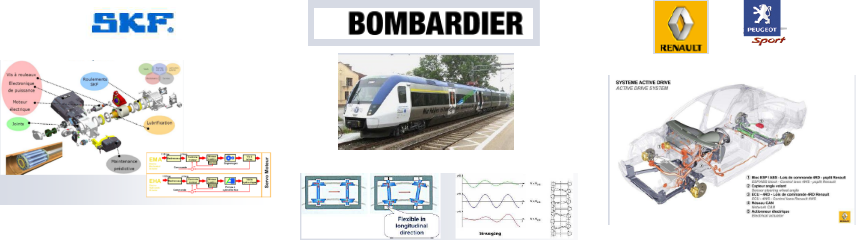
\includegraphics[scale=.4]{./figures/boites_sysml.png}
	\end{block}
}

\frame{
	\frametitle{Qui utilise SysML ?}
	\tiny
	\begin{minipage}[t]{0.48\linewidth}
		\begin{itemize}
			\item "Blohm + Voss Naval GmbH" - bateaux, logistique
			\item "VEGA Space GmbH",- aérospace
			\item "MIT Lincoln Laboratory" - Institute Technologie de Massachusetts
			\item "Lockheed Martin MS2" – militaire
			\item "Lockheed Martin" – militaire
			\item "US Army" – militaire
			\item "ESO - European Organisation for Astronomical Research" – aerospace
			\item "Boeing"
			\item "Raytheon"
			\item "CNES" – France
			\item "Thales" – France
			\item "ESA" - European Space Agency
			\item "NASA"
		\end{itemize}
	\end{minipage}
	\hfill
	\begin{minipage}[t]{0.48\linewidth}
		\begin{itemize}
			\item "BMW"
			\item "Sopra Group" – France
			\item "Thales Security Solutions and Services" – France
			\item "Rockwell Collins Inc."
			\item "JPL" – coentreprise avec la NASA
			\item "GE Aviation"
			\item "GE Transportation" - France, Italie
			\item "NEWTEC LLC"
			\item "NASA Langley Research Center"
			\item "BAE Systems", - France
			\item "Siemens AG"
			\item "Philips"
			\item "NASA Goddard Space Flight Center"
			\item "Bombardier Transportation GmbH"
			\item "Bombardier Transportation Italy"
		\end{itemize}
	\end{minipage}

	\vspace{1em}
	\small ...et bien d'autres !
}

\definecolor{lorange}{RGB}{250,214,185}
\definecolor{lyellow}{RGB}{250,250,100}
\frame{
	\frametitle{SysML, l'ensemble des 9 diagrammes}
	\begin{center}
		\tiny
		\begin{tikzpicture}[scale=.6]
			\draw[drop shadow, fill=lorange] (-2.5,-0.5) rectangle (2.5,0.5);
			\draw (0,0) node{Diagramme SysML};

			\draw[drop shadow, fill=lorange] (-7.5,-1.5) rectangle (-2.5,-2.5);
			\draw (-5,-2) node{Diagramme comportemental};

			\draw[drop shadow, fill=lorange] (7.5,-1.5) rectangle (2.5,-2.5);
			\draw (5,-2) node{Diagramme structurel};

			\draw[drop shadow, fill=lyellow] (-1.5,-1.5) rectangle (1.5,-3);
			\draw (-1.5, -2.5) -- (1.5, -2.5);
			\draw (0,-2) node[align=center]{Diagramme \\ d'exigences};
		\end{tikzpicture}
\end{center}
}
\section[s2]{S2}
\subsection[su1]{SU1}
\frame{
	\frametitle{Contexte}
	\center
	blbl
}
\subsection[su2]{SU2}
\frame{
	\frametitle{Contexte}
	\center
	blbl
}

\end{document}


